\documentclass[12pt]{article}\usepackage[]{graphicx}\usepackage[]{color}
%% maxwidth is the original width if it is less than linewidth
%% otherwise use linewidth (to make sure the graphics do not exceed the margin)
\makeatletter
\def\maxwidth{ %
  \ifdim\Gin@nat@width>\linewidth
    \linewidth
  \else
    \Gin@nat@width
  \fi
}
\makeatother

\definecolor{fgcolor}{rgb}{0.345, 0.345, 0.345}
\newcommand{\hlnum}[1]{\textcolor[rgb]{0.686,0.059,0.569}{#1}}%
\newcommand{\hlstr}[1]{\textcolor[rgb]{0.192,0.494,0.8}{#1}}%
\newcommand{\hlcom}[1]{\textcolor[rgb]{0.678,0.584,0.686}{\textit{#1}}}%
\newcommand{\hlopt}[1]{\textcolor[rgb]{0,0,0}{#1}}%
\newcommand{\hlstd}[1]{\textcolor[rgb]{0.345,0.345,0.345}{#1}}%
\newcommand{\hlkwa}[1]{\textcolor[rgb]{0.161,0.373,0.58}{\textbf{#1}}}%
\newcommand{\hlkwb}[1]{\textcolor[rgb]{0.69,0.353,0.396}{#1}}%
\newcommand{\hlkwc}[1]{\textcolor[rgb]{0.333,0.667,0.333}{#1}}%
\newcommand{\hlkwd}[1]{\textcolor[rgb]{0.737,0.353,0.396}{\textbf{#1}}}%

\usepackage{framed}
\makeatletter
\newenvironment{kframe}{%
 \def\at@end@of@kframe{}%
 \ifinner\ifhmode%
  \def\at@end@of@kframe{\end{minipage}}%
  \begin{minipage}{\columnwidth}%
 \fi\fi%
 \def\FrameCommand##1{\hskip\@totalleftmargin \hskip-\fboxsep
 \colorbox{shadecolor}{##1}\hskip-\fboxsep
     % There is no \\@totalrightmargin, so:
     \hskip-\linewidth \hskip-\@totalleftmargin \hskip\columnwidth}%
 \MakeFramed {\advance\hsize-\width
   \@totalleftmargin\z@ \linewidth\hsize
   \@setminipage}}%
 {\par\unskip\endMakeFramed%
 \at@end@of@kframe}
\makeatother

\definecolor{shadecolor}{rgb}{.97, .97, .97}
\definecolor{messagecolor}{rgb}{0, 0, 0}
\definecolor{warningcolor}{rgb}{1, 0, 1}
\definecolor{errorcolor}{rgb}{1, 0, 0}
\newenvironment{knitrout}{}{} % an empty environment to be redefined in TeX

\usepackage{alltt}
\usepackage{amsmath}
\usepackage{amssymb}
\usepackage{graphicx}
\usepackage{fullpage}
\usepackage{setspace}
\usepackage{hyperref}
\usepackage{color}
\onehalfspacing
\IfFileExists{upquote.sty}{\usepackage{upquote}}{}
\begin{document}

\title{Pol Sci 733: MLE Assignment 1 - Solutions}

\author{Prepared by: Jan Vogler (\href{mailto:jan.vogler@duke.edu}{jan.vogler@duke.edu})}

\date{Grading Due Date: Tuesday, February 2nd, 2016, 3.00 PM}
 
\maketitle



\textbf{\color{red} Insert your comments on the assignment that you are grading above the solution in bold and red text. For example write: ``GRADER COMMENT: everything is correct! - 4/4 Points" Also briefly point out which, if any, problems were not solved correctly and what the mistake was.}

\bigskip

\textbf{Use the following scheme to assign points: For problems that were solved correctly in their entirety, assign the full point value. For correctly solved bonus problems, add that value to the total score for a problem but do not go above the maximum score for each problem. If there are mistakes in the homework, subtract points according to the extent of the mistake. If you subtract points, explain why.}

\bigskip

\textbf{In order to make your text bold and red, you need to insert the following line at the beginning of the document:}

\begin{verbatim} \usepackage{color} \end{verbatim}

\textbf{and the following lines above the solution of the specific task:}

\begin{verbatim} \textbf{\color{red} GRADER COMMENT: everything is correct! - 4/4 Points} \end{verbatim}



\pagebreak

\section*{Problem 1 (5 points)}

Given is the probability density function of the exponential distribution for a single observation:

\bigskip

$f(x) = \lambda * exp(-\lambda*x)$

\bigskip

In order to find the MLE for $\lambda$, we first treat the value of our observation (X=x) as fixed, which means that we now have a function of $\lambda$.

\bigskip

$L(\lambda | X = x) = L(\lambda) = \lambda * exp(-\lambda*x)$

\bigskip

Next, we take the natural logarithm of this function:

\bigskip

$\log(L(\lambda))) = \log(\lambda) - \lambda *x$

\bigskip

Taking the derivative of this function is easy:

\bigskip

$\dfrac{d \log(L(\lambda))}{d \lambda} = \dfrac{1}{\lambda} - x$

\bigskip

If we set this to zero, we find that:

\bigskip

$\hat{\lambda} = \dfrac{1}{x}$

\bigskip

We still need to verify that the second derivative is negative, so:

\bigskip

$\dfrac{d^2 \log(L(\lambda))}{d \lambda^2} = - \dfrac{1}{\lambda^2}$

\bigskip

$- \dfrac{1}{\lambda^2}$ is negative for all values of $x > 0$ because $\hat{\lambda} = \dfrac{1}{x}$. Accordingly, we have found a maximum.

\bigskip

The solution for multiple draws from the exponential distribution is:

\bigskip

$L(\lambda | X = x_1, ..., x_n) = L(\lambda) = \lambda ^n * exp(-\lambda*\sum_{i=1}^{n} x_i)$

\bigskip

$\log(L(\lambda))) = n * \log(\lambda) - \lambda * \sum_{i=1}^{n} x_i$

\bigskip

$\dfrac{d \log(L(\lambda))}{d \lambda} = \dfrac{n}{\lambda} - \sum_{i=1}^{n} x_i = 0$

\bigskip

$\hat{\lambda} = \dfrac{n}{\sum_{i=1}^{n} x_i}$

\bigskip

The second derivative in this case is:

\bigskip

$\dfrac{d^2 \log(L(\lambda))}{d \lambda^2} = - \dfrac{n}{\lambda^2}$

\bigskip

Which is also negative for all values of $\hat{\lambda} = \dfrac{n}{\sum_{i=1}^{n} x_i}$ where $\sum_{i=1}^{n} x_i > 0$, so we found a maximum.



\section*{Problem 2 (5 points)}

The second problem requires us to find the variance of the MLE $\hat{\lambda}$.

If we find the MLE by setting the first derivative to zero, we can find the variance of the MLE through Fisher's information $I(\hat{\lambda})$.

To be precise:

\bigskip

$\hat{\lambda} \sim Normal(\lambda,\dfrac{\tau^2}{n})$

\bigskip

Where:

\bigskip

$\tau^2 =  \dfrac{1}{I(\hat{\lambda})}$

\bigskip

Fortunately, we have already calculated the second derivative of the log-likelihood for a single observation (which is the one required to find Fisher's information), which was:

\bigskip

$\dfrac{d^2 \log(L(\lambda))}{d \lambda^2} = - \dfrac{1}{\lambda^2}$.

\bigskip

$I(\hat{\lambda})$ is equivalent to $- E(\dfrac{d^2 \log(L(\lambda))}{d \lambda^2})$.

\bigskip

In this case:

\bigskip

$- E(- \dfrac{1}{\lambda^2})$, which is $\dfrac{1}{\lambda^2}$.

\bigskip

This means that:

\bigskip

$I(\hat{\lambda}) = \dfrac{1}{\lambda^2} \Rightarrow \tau^2 = \lambda^2$

\bigskip

Therefore, the estimator is distributed as a Normal with the following properties:

\bigskip

$\hat{\lambda} \sim Normal(\lambda,\dfrac{\lambda^2}{n})$

\bigskip

As $n = 1$, we know that the variance is $\lambda^2$. For multiple draws, the variance simply is $\dfrac{\lambda^2}{n}$.



\section*{Problem 3 (6 points)}

\textbf{Graders, please do not subtract any points if someone has not included the graphics. The homework does not require the inclusion of graphics.}

\subsection*{a)}

\begin{knitrout}
\definecolor{shadecolor}{rgb}{0.969, 0.969, 0.969}\color{fgcolor}\begin{kframe}
\begin{alltt}
\hlcom{# Simulate 100 data points from exponential distribution with rate 0.5}

\hlkwd{set.seed}\hlstd{(}\hlnum{2}\hlstd{)}
\hlstd{simdata} \hlkwb{=} \hlkwd{rexp}\hlstd{(}\hlnum{100}\hlstd{,} \hlkwc{rate} \hlstd{=} \hlnum{0.5}\hlstd{)}
\hlkwd{summary}\hlstd{(simdata)}
\end{alltt}
\begin{verbatim}
##    Min. 1st Qu.  Median    Mean 3rd Qu.    Max. 
## 0.00788 0.68320 1.64900 2.01300 2.58600 9.72400
\end{verbatim}
\begin{alltt}
\hlkwd{hist}\hlstd{(simdata)}
\end{alltt}
\end{kframe}
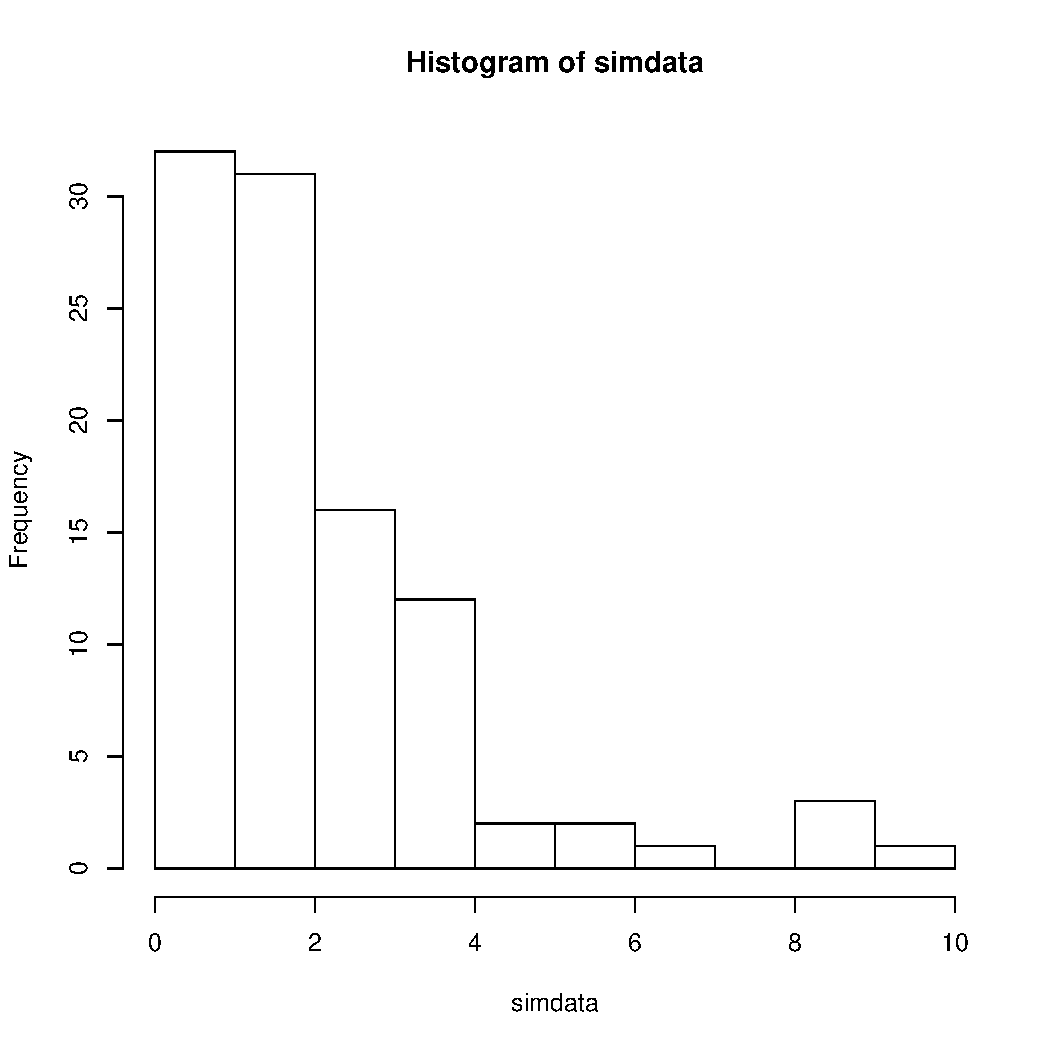
\includegraphics[width=\maxwidth]{figure/unnamed-chunk-1-1} 

\end{knitrout}

\subsection*{b)}

\begin{knitrout}
\definecolor{shadecolor}{rgb}{0.969, 0.969, 0.969}\color{fgcolor}\begin{kframe}
\begin{alltt}
\hlcom{# Declare log-likelihood function in general terms}

\hlstd{LL_exponential} \hlkwb{<-} \hlkwa{function}\hlstd{(}\hlkwc{rate}\hlstd{,} \hlkwc{data}\hlstd{) \{}
    \hlopt{-}\hlkwd{sum}\hlstd{(}\hlkwd{dexp}\hlstd{(data, rate,} \hlkwc{log} \hlstd{=} \hlnum{TRUE}\hlstd{))}  \hlcom{#We take the negative of the sum because the optimizer in 'mle2' finds the minimum of a function}
\hlstd{\}}
\end{alltt}
\end{kframe}
\end{knitrout}

\subsection*{c)}

\begin{knitrout}
\definecolor{shadecolor}{rgb}{0.969, 0.969, 0.969}\color{fgcolor}\begin{kframe}
\begin{alltt}
\hlcom{# Load required package}
\hlkwd{library}\hlstd{(bbmle)}
\end{alltt}


{\ttfamily\noindent\itshape\color{messagecolor}{\#\# Loading required package: stats4}}\begin{alltt}
\hlcom{# Optimize given the observed data}

\hlstd{fit} \hlkwb{<-} \hlkwd{mle2}\hlstd{(LL_exponential,} \hlkwc{start} \hlstd{=} \hlkwd{list}\hlstd{(}\hlkwc{rate} \hlstd{=} \hlnum{1}\hlstd{),} \hlkwc{data} \hlstd{=} \hlkwd{list}\hlstd{(}\hlkwc{data} \hlstd{= simdata))}
\end{alltt}


{\ttfamily\noindent\color{warningcolor}{\#\# Warning in dexp(data, rate, log = TRUE): NaNs produced}}

{\ttfamily\noindent\color{warningcolor}{\#\# Warning in dexp(data, rate, log = TRUE): NaNs produced}}

{\ttfamily\noindent\color{warningcolor}{\#\# Warning in dexp(data, rate, log = TRUE): NaNs produced}}\end{kframe}
\end{knitrout}

\subsection*{d)}

\begin{knitrout}
\definecolor{shadecolor}{rgb}{0.969, 0.969, 0.969}\color{fgcolor}\begin{kframe}
\begin{alltt}
\hlcom{# Report estimates and uncertainty bounds}

\hlkwd{summary}\hlstd{(fit)}
\end{alltt}
\begin{verbatim}
## Maximum likelihood estimation
## 
## Call:
## mle2(minuslogl = LL_exponential, start = list(rate = 1), data = list(data = simdata))
## 
## Coefficients:
##      Estimate Std. Error z value     Pr(z)    
## rate 0.496622   0.049662      10 < 2.2e-16 ***
## ---
## Signif. codes:  0 '***' 0.001 '**' 0.01 '*' 0.05 '.' 0.1 ' ' 1
## 
## -2 log L: 339.9707
\end{verbatim}
\begin{alltt}
\hlkwd{confint}\hlstd{(fit)}
\end{alltt}
\begin{verbatim}
##     2.5 %    97.5 % 
## 0.4055838 0.6004699
\end{verbatim}
\end{kframe}
\end{knitrout}

\subsection*{e)}

\begin{knitrout}
\definecolor{shadecolor}{rgb}{0.969, 0.969, 0.969}\color{fgcolor}\begin{kframe}
\begin{alltt}
\hlcom{# One-tailed Wald test for null hypothesis rate = 0.75}

\hlstd{wald} \hlkwb{<-} \hlkwd{abs}\hlstd{(}\hlkwd{coef}\hlstd{(fit)[}\hlnum{1}\hlstd{]} \hlopt{-} \hlnum{0.75}\hlstd{)}\hlopt{/}\hlkwd{sqrt}\hlstd{(}\hlkwd{vcov}\hlstd{(fit))}
\hlstd{wald}
\end{alltt}
\begin{verbatim}
##          rate
## rate 5.102027
\end{verbatim}
\begin{alltt}
\hlkwd{curve}\hlstd{(}\hlkwd{dnorm}\hlstd{(x,} \hlnum{0}\hlstd{,} \hlnum{1}\hlstd{),} \hlkwc{from} \hlstd{=} \hlopt{-}\hlnum{10}\hlstd{,} \hlkwc{to} \hlstd{=} \hlnum{10}\hlstd{)}
\hlkwd{abline}\hlstd{(}\hlkwc{v} \hlstd{= wald,} \hlkwc{lty} \hlstd{=} \hlnum{2}\hlstd{)}
\end{alltt}
\end{kframe}
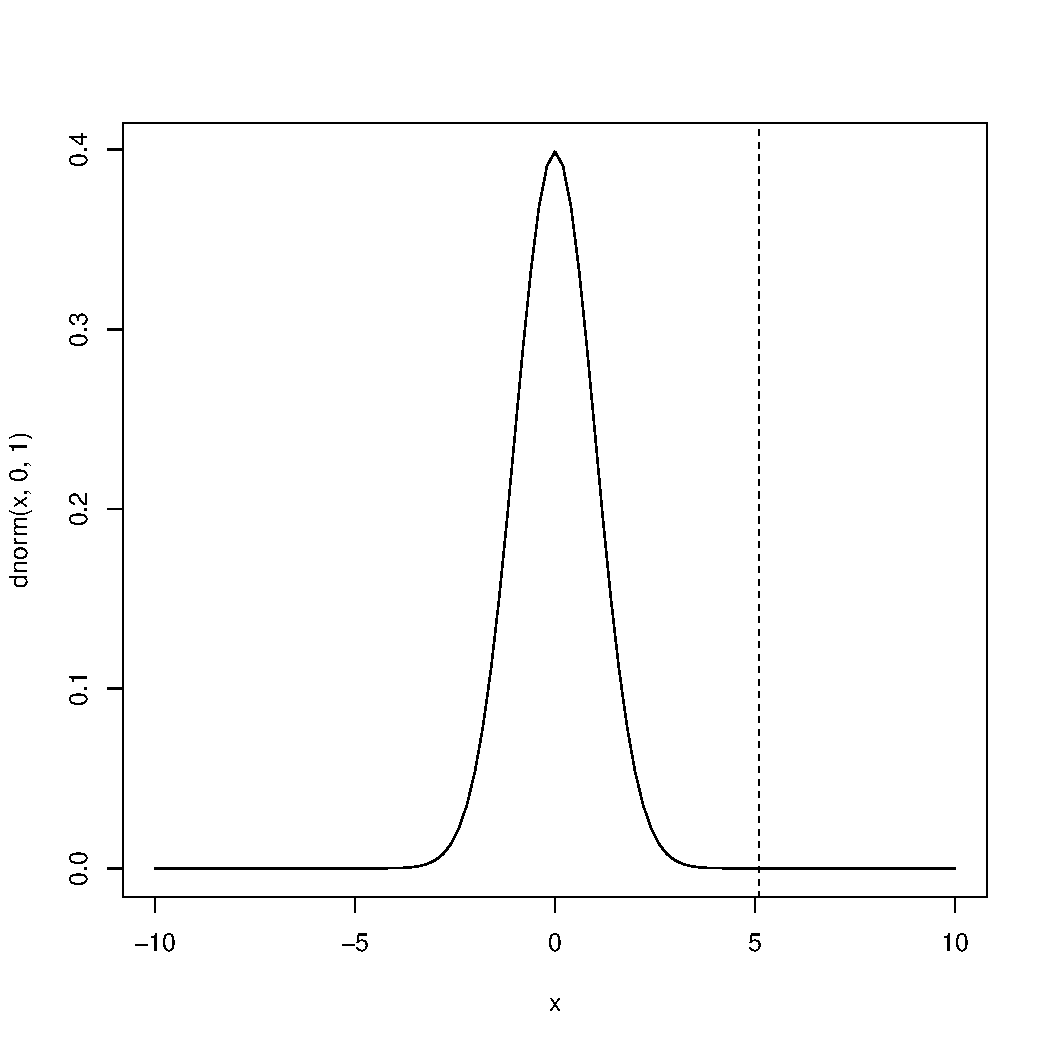
\includegraphics[width=\maxwidth]{figure/unnamed-chunk-5-1} 
\begin{kframe}\begin{alltt}
\hlnum{1} \hlopt{-} \hlkwd{pnorm}\hlstd{(wald)}
\end{alltt}
\begin{verbatim}
##              rate
## rate 1.680173e-07
\end{verbatim}
\begin{alltt}
\hlcom{# Two-tailed Wald test for null hypothesis rate = 0.75}

\hlnum{1} \hlopt{-} \hlkwd{pnorm}\hlstd{(wald)} \hlopt{+} \hlkwd{pnorm}\hlstd{(}\hlopt{-}\hlstd{wald)}
\end{alltt}
\begin{verbatim}
##              rate
## rate 3.360346e-07
\end{verbatim}
\end{kframe}
\end{knitrout}

\subsection*{f)}

\begin{knitrout}
\definecolor{shadecolor}{rgb}{0.969, 0.969, 0.969}\color{fgcolor}\begin{kframe}
\begin{alltt}
\hlcom{# One-tailed likelihood ratio test comparing fit model with null model}

\hlstd{fit_null} \hlkwb{<-} \hlkwd{mle2}\hlstd{(LL_exponential,} \hlkwc{start} \hlstd{=} \hlkwd{list}\hlstd{(),} \hlkwc{fixed} \hlstd{=} \hlkwd{list}\hlstd{(}\hlkwc{rate} \hlstd{=} \hlnum{0.75}\hlstd{),}
    \hlkwc{data} \hlstd{=} \hlkwd{list}\hlstd{(}\hlkwc{data} \hlstd{= simdata))}

\hlkwd{summary}\hlstd{(fit_null)}
\end{alltt}
\begin{verbatim}
## Maximum likelihood estimation
## 
## Call:
## mle2(minuslogl = LL_exponential, start = list(), fixed = list(rate = 0.75), 
##     data = list(data = simdata))
## 
## Coefficients:
##      Estimate Std. Error z value Pr(z)
## 
## -2 log L: 359.5551
\end{verbatim}
\begin{alltt}
\hlkwd{summary}\hlstd{(fit)}
\end{alltt}
\begin{verbatim}
## Maximum likelihood estimation
## 
## Call:
## mle2(minuslogl = LL_exponential, start = list(rate = 1), data = list(data = simdata))
## 
## Coefficients:
##      Estimate Std. Error z value     Pr(z)    
## rate 0.496622   0.049662      10 < 2.2e-16 ***
## ---
## Signif. codes:  0 '***' 0.001 '**' 0.01 '*' 0.05 '.' 0.1 ' ' 1
## 
## -2 log L: 339.9707
\end{verbatim}
\begin{alltt}
\hlcom{# Easy and quick calculation of the LR test}

\hlstd{lrtest} \hlkwb{=} \hlnum{359.5551} \hlopt{-} \hlnum{339.9707}
\hlstd{lrtest}
\end{alltt}
\begin{verbatim}
## [1] 19.5844
\end{verbatim}
\begin{alltt}
\hlcom{# Alternative calculation of LR test (just for demonstration purposes)}

\hlcom{# First find the original likelihoods}
\hlstd{lnull} \hlkwb{=} \hlkwd{exp}\hlstd{(}\hlopt{-}\hlnum{0.5} \hlopt{*} \hlstd{(}\hlnum{359.5551}\hlstd{))}
\hlstd{lalt} \hlkwb{=} \hlkwd{exp}\hlstd{(}\hlopt{-}\hlnum{0.5} \hlopt{*} \hlstd{(}\hlnum{339.9707}\hlstd{))}

\hlstd{lnull}
\end{alltt}
\begin{verbatim}
## [1] 8.386912e-79
\end{verbatim}
\begin{alltt}
\hlstd{lalt}
\end{alltt}
\begin{verbatim}
## [1] 1.500723e-74
\end{verbatim}
\begin{alltt}
\hlcom{# Original LR test formula}

\hlstd{lrtest2} \hlkwb{=} \hlopt{-}\hlnum{2} \hlopt{*} \hlkwd{log}\hlstd{(lnull}\hlopt{/}\hlstd{lalt)}
\hlstd{lrtest2}
\end{alltt}
\begin{verbatim}
## [1] 19.5844
\end{verbatim}
\begin{alltt}
\hlcom{# Plug into curve}

\hlkwd{curve}\hlstd{(}\hlkwd{dchisq}\hlstd{(x,} \hlnum{1}\hlstd{),} \hlkwc{from} \hlstd{=} \hlnum{0}\hlstd{,} \hlkwc{to} \hlstd{=} \hlnum{100}\hlstd{)}
\hlkwd{abline}\hlstd{(}\hlkwc{v} \hlstd{= lrtest,} \hlkwc{lty} \hlstd{=} \hlnum{2}\hlstd{)}
\end{alltt}
\end{kframe}
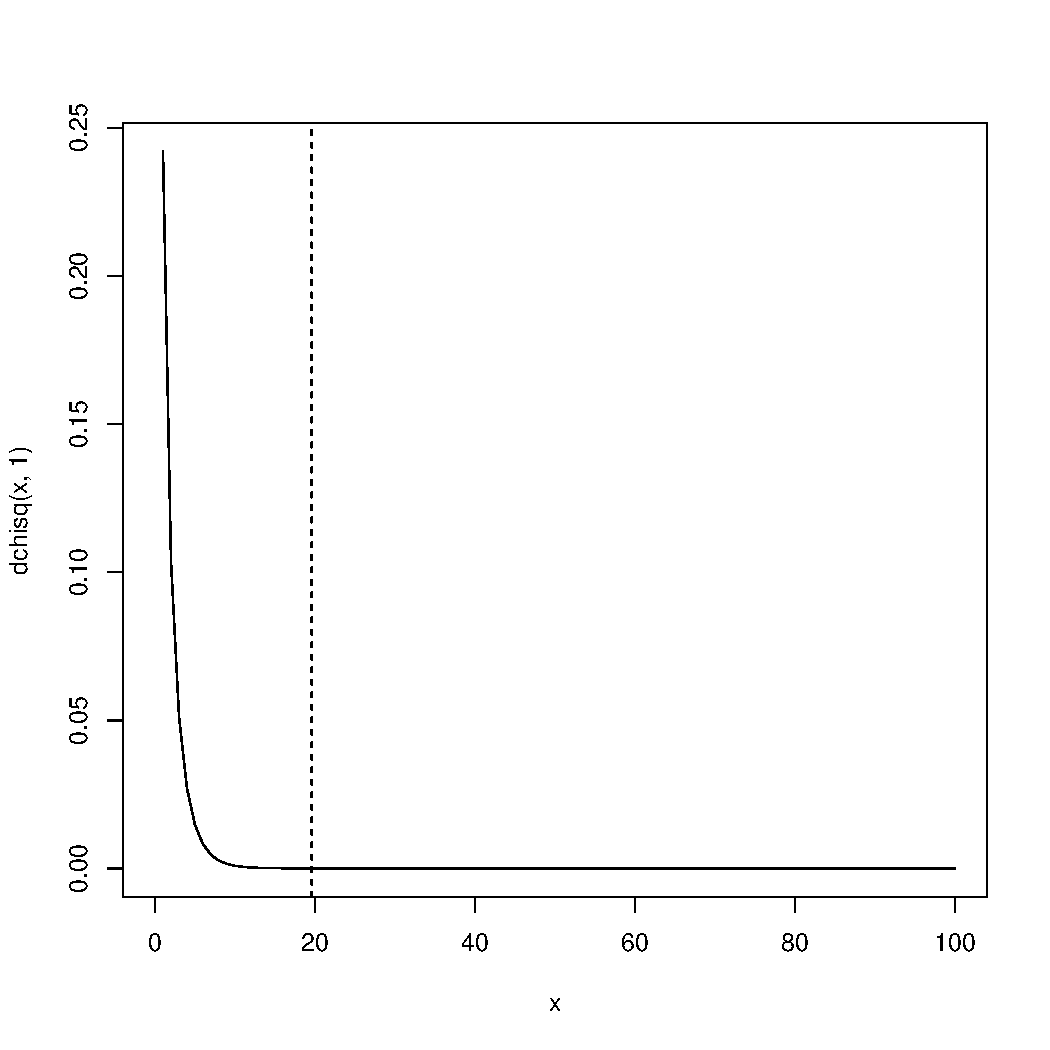
\includegraphics[width=\maxwidth]{figure/unnamed-chunk-6-1} 
\begin{kframe}\begin{alltt}
\hlnum{1} \hlopt{-} \hlkwd{pchisq}\hlstd{((lrtest),} \hlnum{1}\hlstd{)}
\end{alltt}
\begin{verbatim}
## [1] 9.625191e-06
\end{verbatim}
\end{kframe}
\end{knitrout}



\end{document}
